%!Mode:: "TeX:UTF-8"
\section{服务器集群}

一个完整的负载均衡项目,一般由虚拟服务器、故障隔离及失败切换3个功能框架所组成。

\begin{figure}[ht]
	\begin{center}
		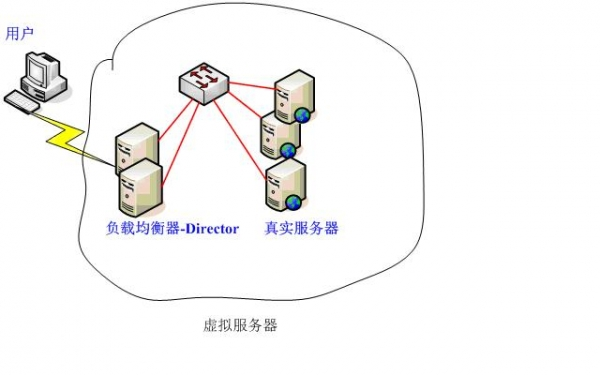
\includegraphics[keepaspectratio,width=0.5\paperwidth]{Pictures/Network/VirtualServer.jpg}
	\caption{虚拟服务器}
	\label{fig:VirtualServer}
	\end{center}
\end{figure}

虚拟服务器是负载均衡体系的基本架构,它分两层结构:转发器(Director)和真实服务器。图\ref{fig:VirtualServer}为虚拟服务器的结构示意。

为什么称虚拟服务器?因为从用户的角度看来,似乎只是一个服务器在提供服务。虚拟服务器最主要的功能是提供包转发和负载均衡,这个功能可以通过撰写ipvsadm脚本具体实现。虚拟服务器项目由章文嵩博士所贡献,目前已被添加到各种Linux发行版的内核。

故障隔离指虚拟服务器中的某个真实服务器(或某几个真实服务器)失效或发生故障,系统将自动把失效的服务器从转发队列中清理出去,从而保证用户访问的正确性;另一方面,当实效的服务器被修复以后,系统再自动地把它加入转发队列。

失败切换,这是针对负载均衡器Director采取的措施,在有两个负载均衡器Director的应用场景,当主负载均衡器(MASTER)失效或出现故障,备份负载均衡器(BACKUP)将自动接管主负载均衡器的工作;一旦主负载均衡器故障修复,两者将恢复到最初的角色。

要从技术上实现虚拟服务器、故障隔离及失败切换3个功能,需要两个工具:ipvsadm和keepalived。当然也有heartbeat这样的工具可以实现同样的功能,但相对于keepalived,heartbeat的实现要复杂得多(如撰写ipvsadm脚本,部署ldirectord,编写资源文件等)。在采用keepalived的方案里,只要ipvsadm被正确的安装,简单的配置唯一的文件keepalived就行了。


\subsection{LVS}
LVS是Linux Virtual Server的简写,意即Linux虚拟服务器,是一个虚拟的服务器集群系统。本项目在1998年5月由章文嵩博士成立,是中国国内最早出现的自由软件项目之一。

\begin{figure}[ht]
	\begin{center}
		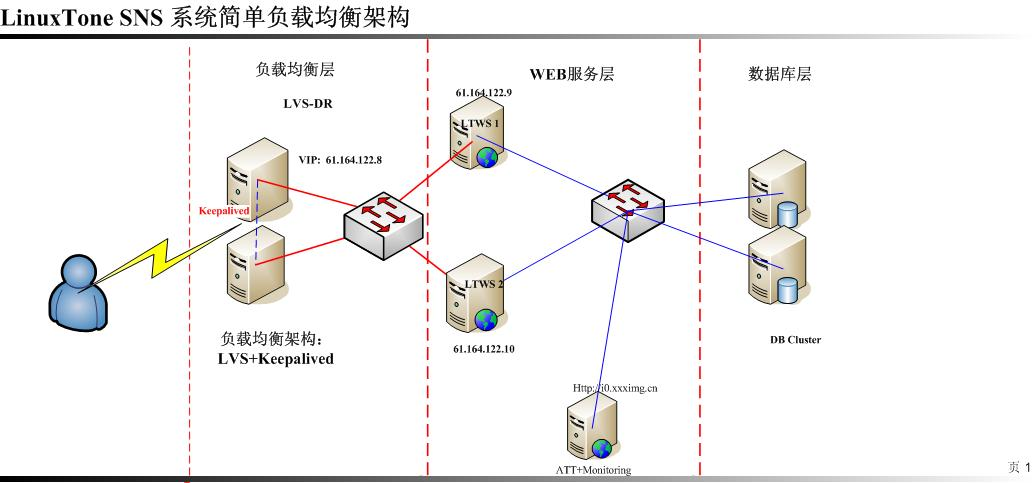
\includegraphics[keepaspectratio,width=0.5\paperwidth]{Pictures/Network/LinuxToneSnsArch.jpg}
	\caption{LinuxTone网站架构}
	\label{fig:LinuxToneSnsArch}
	\end{center}
\end{figure}

LVS常常与keepalived进行协作,如图\ref{fig:LinuxToneSnsArch}所示。


LVS集群采用IP负载均衡技术和基于内容请求分发技术。调度器具有很好的吞吐率,将请求均衡地转移到不同的服务器上执行,且调度器自动屏蔽掉服务器的故障,从而将一组服务器构成一个高性能的、高可用的虚拟服务器。整个服务器集群的结构对客户是透明的,而且无需修改客户端和服务器端的程序。为此,在设计时需要考虑系统的透明性、可伸缩性、高可用性和易管理性。
目前有三种IP负载均衡技术\textbf{(VS/NAT、VS/TUN和VS/DR)}。

一般来说,LVS集群采用三层结构,其主要组成部分为:
\begin{description}
\item[负载调度器(load balancer)] 它是整个集群对外面的前端机,它可以采用IP负载均衡技术、基于内容请求分发技术或者两者相结合
\item[服务器池(server pool)] 是一组真正执行客户请求的服务器,执行的服务有WEB、MAIL、FTP和DNS等
\item[共享存储(shared storage)] 它为服务器池提供一个共享的存储区,这样很容易使得服务器池拥有相同的内容,提供相同的服务
\end{description}


\subsection{IPVS}
IPVS(IP Virtual Server)是运行在LVS下的提供负载平衡功能的一种技术。

IPVS基本上是一种高效的Layer-4交换机,它提供负载平衡的功能。当一个TCP连接的初始SYN报文到达时,IPVS就选择一台服务器,将报文转发给它。此后通过查发报文的IP和TCP报文头地址,保证此连接的后继报文被转发到相同的服务器。这样,IPVS无法检查到请求的内容再选择服务器,这就要求后端的服务器组是提供相同的服务,不管请求被送到哪一台服务器,返回结果都应该是一样的。但是在有一些应用中后端的服务器可能功能不一,有的是提供HTML文档的Web服务器,有的是提供图片的Web服务器,有的是提供CGI的Web服务器。这时,就需要基于内容请求分发 (Content-Based Request Distribution),同时基于内容请求分发可以提高后端服务器上访问的局部性。

LVS的IP负载平衡技术就是通过IPVS模块来实现的,IPVS是LVS集群系统的核心软件,它的主要作用是:安装在Director Server上,同时在Director Server上虚拟出一个IP地址,用户必须通过这个虚拟的IP地址访问服务。这个虚拟IP一般称为LVS的VIP,即Virtual IP。访问的请求首先经过VIP到达负载调度器,然后由负载调度器从Real Server列表中选取一个服务节点响应用户的请求。

\subsection{Keepalived}
keepalived是一款失效转发机制的软件, 它的作用是检测web服务器的状态,如果有一台web服务器死机,或工作出现故障,Keepalived将检测到,并将有故障的web服务器从系统中剔除,当web服务器工作正常后Keepalived自动将web服务器加入到服务器群中,这些工作全部自动完成,不需要人工干涉,需要人工做的只是修复故障的web服务器。

网络在设计的时候必须考虑到冗余容灾,包括线路冗余,设备冗余等,防止网络存在单点故障,那在路由器或三层交换机处实现冗余就显得尤为重要,在网络里面有个协议就是来做这事的,这个协议就是VRRP协议,Keepalived就是巧用VRRP协议来实现高可用性(HA)的。keepalived完全遵守VRRP协议,包括竞选机制等等。


\begin{figure}[ht]
	\begin{center}
		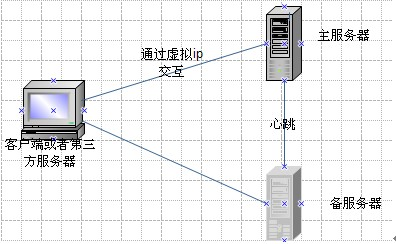
\includegraphics[keepaspectratio,width=0.5\paperwidth]{Pictures/Network/keepalivedIllus.jpg}
	\caption{Keepalived工作原理}
	\label{fig:keepalivedIllus}
	\end{center}
\end{figure}

图\ref{fig:keepalivedIllus}中主服务器和备服务器都装了keepalived软件,将keepalived配置成Master的便成了主服务器,将keepaliv-ed配置成BACKUP的自然就成了备服务器。主备服务器都通过keepalived绑定有相同的虚拟ip,外界就是利用这个虚拟ip与服务器进行交互的。正常情况下只有主服务器work,当主服务器宕机或者出现其他故障时Keepalived会将work转移到备服务器上,虚拟ip依然有效。当主服务器修复好了备用服务器会自动将work权利重新交给主服务器。 

keepalived也是模块化设计,不同模块复杂不同的功能,下面是keepalived的组件:

\begin{description}
\item[core]是keepalived的核心,复杂主进程的启动和维护,全局配置文件的加载解析等
\item[check]负责healthchecker(健康检查),包括了各种健康检查方式,以及对应的配置的解析包括LVS的配置解析
\item[vrrp]VRRPD子进程,VRRPD子进程就是来实现VRRP协议的
\item[libipfwc]iptables(ipchains)库,配置LVS会用到
\item[libipvs]配置LVS会用到
\end{description}

\begin{figure}[ht]
	\begin{center}
		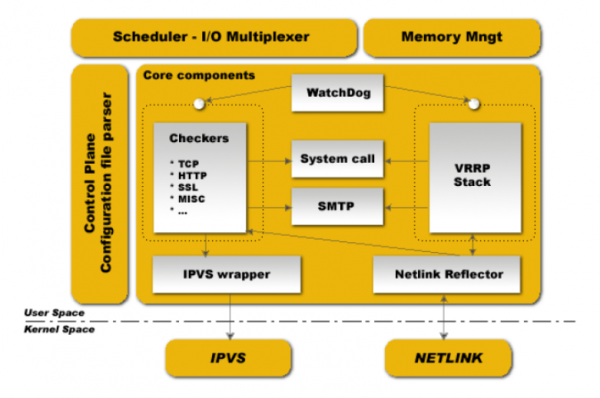
\includegraphics[keepaspectratio,width=0.5\paperwidth]{Pictures/Network/KeepalivedCore.png}
	\caption{Keepalived内部架构}
	\label{fig:KeepalivedCore}
	\end{center}
\end{figure}

keepalived启动后会有三个进程。父进程负责内存管理,子进程管理等等,两个子进程分别运行VRRP和healthchecker。
被系统WatchDog看管,healthchecker子进程复杂检查各自服务器的健康程度,例如HTTP,LVS等等,如果healthchecker子进程检查到MASTER上服务不可用了,就会通知本机上的兄弟VRRP子进程,让他删除通告,并且去掉虚拟IP,转换为BACKUP。

\subsection{Watchdog}

Carrier Grade Linux 是 OSDL(Open Source Development Lab)发布的电信级 Linux 的标准,在系统可用性这部分指出Linux必须支持 watchdog 机制。

Watchdog在实现上可以是硬件电路也可以是软件定时器,能够在系统出现故障时自动重新启动系统。在Linux 内核下, watchdog的基本工作原理是:当watchdog启动后(即/dev/watchdog 设备被打开后),如果在某一设定的时间间隔内/dev/watchdog没有被执行写操作, 硬件watchdog电路或软件定时器就会重新启动系统。

/dev/watchdog 是一个主设备号为10, 从设备号130的字符设备节点。 Linux内核不仅为各种不同类型的watchdog硬件电路提供了驱动,还提供了一个基于定时器的纯软件watchdog驱动。 驱动源码位于内核源码树drivers/char/watchdog/目录下。


\subsection{Memcached}

memcached是一套分布式的高速缓存系统,由LiveJournal的Brad Fitzpatrick开发,但目前被许多网站使用。这是一套开放源代码软件,以BSD license授权发布。

memcached缺乏认证以及安全管制,这代表应该将memcached服务器放置在防火墙后。

memcached的API使用三十二比特的循环冗余校验(CRC-32)计算键值后,将数据分散在不同的机器上。当表格满了以后,接下来新增的数据会以LRU机制替换掉。由于memcached通常只是当作高速缓存系统使用,所以使用memcached的应用程序在写回较慢的系统时(像是后端的数据库)需要额外的代码更新memcached内的数据。


\clearpage